\section{Conclusions}
\label{sec:discussion-conclusion}
The general objective is to classify objects and materials, where a version with each material feature of each object exists.
Those objects are visualized with 12 views from different perspectives.
Grouping those views regarding their discrimination is supposed to increase the performance, hence, it is building the core functionality of the presented network architecture.
Each discrimination is represented by a view discrimination score that is a single number calculated by a fully-connected layer with a view descriptor as input.
Here the last view descriptor from the fifth convolutional layer is chosen, that is the last one in the network because it resembles the most accurate features of a view.
Depending on their scores, the views are divided in 12 uniformly distributed groups for having the most flexibility.
For each group, a view descriptor is generated by averaging its contained view descriptors.
This is possible because the views of each group have probably similar features, thus, they are combined equally.
Each group gets a weight associated that is the average of its included view discrimination scores.
Then each single group descriptor is propagated through two fully-connected layers generating a shape descriptor for the particular group.
Hence, the output of the seventh layer are shape descriptors.
With those group shape descriptors, a weighted average is calculated using each related group weight.
This generates a single shape descriptor describing the actual object.
Propagating this through the last fully-connected layer, the eighth one, yields the prediction of the network.
Combining this with a softmax layer yields the prediction probabilities for the classes.
A summary of the layers is given in \tabref{tab:network-layers}.

For the grouping mechanism, the following results are observed.
The 0-3 network treats views with a visible material feature the most discriminative.
However, those discriminations are reduced drastically when more material features are added and mostly views showing no material feature are preferred for discrimination.
Moreover, by comparing equivalent material classes but with a different color like green to red or green-green to red-red it is shown, that each score differs.
Hence, the assumption is postulated that for each material class a range of values for the final shape descriptor is defined.
Depending on how large it is a particular material class is predicted.

The minimum losses and maximum accuracies during the training process of all networks are visualized in \figref{fig:losses} and \figref{fig:accuracies}.
The corresponding values are noted in \tabref{tab:network-performances}.
With the addition of material features the networks get more complicated, hence their loss increases and the accuracy decreases.
It is noticeable, that using 5 or 6 material classes, wrong predictions are very likely to be within the same category but with the related single or double feature of the same color.
This can presumably be coped by a larger dataset or a longer training due to no indicator of overfitting.
The first simulates the latter by having more batches, thus more updates are performed on the parameters.
For the losses it can be seen, that for the single-category networks they are similar for training and testing set.
However, the ones for the four-category losses differ extremely.
Those training losses are much smaller than the ones from the single-category networks, though.
The smaller losses are presumably due to the larger datasets.
The difference between training losses and testing losses is supposedly due to the different cost functions of both sets.
Because the cost function of the four-category networks is way more complex than the one of the single-category networks by having more extrema.
If now well-suited parameters for the training set are found, they do not necessarily represent a well-suited point in the testing cost function as illustrated in \figref{fig:sgdr-cost}.
This can be overcome by finding a broader minimum.
It is difficult to compare the networks to recent researches because their objective is different.
However, the closest one to the MVCNN and GVCNN results is the 4-0 network, because it uses classes from the ModelNet10 dataset and no material features.
The first one reaches an accuracy of 89.9\% taking the network with the closest configuration as a reference.
This was improved to 95.0\% by \textit{Su et al}.
The GVCNN reaches an accuracy of 92.6\%.
However, all of them use the ModelNet40 as a benchmark, so the results are not fully comparable but indicate the right direction.
\begin{figure}
	\setlength\figureheight{.4\textwidth}
	\setlength\figurewidth{.8\textwidth}
	\centering
	%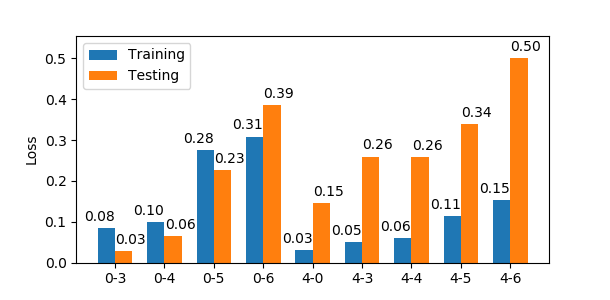
\includegraphics[]{images/conclusion_loss.png}
	% This file was created by matplotlib2tikz v0.7.3.
\begin{tikzpicture}

\definecolor{color0}{rgb}{0.12156862745098,0.466666666666667,0.705882352941177}
\definecolor{color1}{rgb}{1,0.498039215686275,0.0549019607843137}

\begin{axis}[
height=\figureheight,
legend cell align={left},
legend style={at={(0.03,0.97)}, anchor=north west, draw=white!80.0!black},
tick align=outside,
tick pos=left,
width=\figurewidth,
x grid style={white!69.01960784313725!black},
xmin=-0.785, xmax=8.785,
xtick style={color=black},
xtick={0,1,2,3,4,5,6,7,8},
xticklabels={0-3,0-4,0-5,0-6,4-0,4-3,4-4,4-5,4-6},
y grid style={white!69.01960784313725!black},
ylabel={Loss},
ymin=0, ymax=0.52495015965173,
ytick style={color=black},
ytick={0,0.1,0.2,0.3,0.4,0.5,0.6},
yticklabels={0.0,0.1,0.2,0.3,0.4,0.5,}
]
\draw[fill=color0,draw opacity=0] (axis cs:-0.35,0) rectangle (axis cs:0,0.0848326952661315);
\addlegendimage{ybar,ybar legend,fill=color0,draw opacity=0};
\addlegendentry{Training}

\draw[fill=color0,draw opacity=0] (axis cs:0.65,0) rectangle (axis cs:1,0.0985216816457418);
\draw[fill=color0,draw opacity=0] (axis cs:1.65,0) rectangle (axis cs:2,0.275235192127982);
\draw[fill=color0,draw opacity=0] (axis cs:2.65,0) rectangle (axis cs:3,0.308308220500576);
\draw[fill=color0,draw opacity=0] (axis cs:3.65,0) rectangle (axis cs:4,0.0313814810523625);
\draw[fill=color0,draw opacity=0] (axis cs:4.65,0) rectangle (axis cs:5,0.0493501171798515);
\draw[fill=color0,draw opacity=0] (axis cs:5.65,0) rectangle (axis cs:6,0.0601031640727976);
\draw[fill=color0,draw opacity=0] (axis cs:6.65,0) rectangle (axis cs:7,0.114382526963265);
\draw[fill=color0,draw opacity=0] (axis cs:7.65,0) rectangle (axis cs:8,0.152284982224603);
\draw[fill=color1,draw opacity=0] (axis cs:0,0) rectangle (axis cs:0.35,0.0273379426863458);
\addlegendimage{ybar,ybar legend,fill=color1,draw opacity=0};
\addlegendentry{Testing}

\draw[fill=color1,draw opacity=0] (axis cs:1,0) rectangle (axis cs:1.35,0.0646619006853413);
\draw[fill=color1,draw opacity=0] (axis cs:2,0) rectangle (axis cs:2.35,0.226243400408162);
\draw[fill=color1,draw opacity=0] (axis cs:3,0) rectangle (axis cs:3.35,0.385673365935131);
\draw[fill=color1,draw opacity=0] (axis cs:4,0) rectangle (axis cs:4.35,0.145997776799723);
\draw[fill=color1,draw opacity=0] (axis cs:5,0) rectangle (axis cs:5.35,0.259522616167633);
\draw[fill=color1,draw opacity=0] (axis cs:6,0) rectangle (axis cs:6.35,0.257949455544197);
\draw[fill=color1,draw opacity=0] (axis cs:7,0) rectangle (axis cs:7.35,0.339136986151614);
\draw[fill=color1,draw opacity=0] (axis cs:8,0) rectangle (axis cs:8.35,0.499952533001647);
\end{axis}

\end{tikzpicture}
	\caption{Losses of all networks}
	\label{fig:losses}
\end{figure}
\begin{figure}
	\setlength\figureheight{.4\textwidth}
	\setlength\figurewidth{.8\textwidth}
	\centering
	%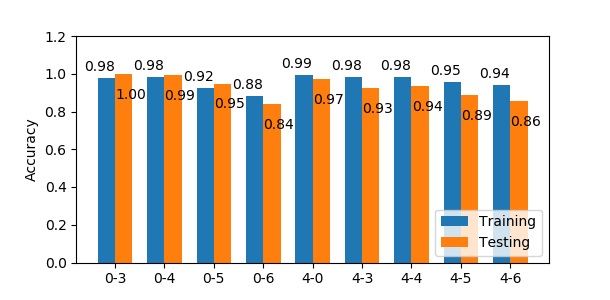
\includegraphics[]{images/conclusion_accuracy.png}
	% This file was created by matplotlib2tikz v0.7.3.
\begin{tikzpicture}

\definecolor{color0}{rgb}{0.12156862745098,0.466666666666667,0.705882352941177}
\definecolor{color1}{rgb}{1,0.498039215686275,0.0549019607843137}

\begin{axis}[
height=\figureheight,
legend cell align={left},
legend style={at={(0.97,0.03)}, anchor=south east, draw=white!80.0!black},
tick align=outside,
tick pos=left,
width=\figurewidth,
x grid style={white!69.01960784313725!black},
xmin=-0.785, xmax=8.785,
xtick style={color=black},
xtick={0,1,2,3,4,5,6,7,8},
xticklabels={0-3,0-4,0-5,0-6,4-0,4-3,4-4,4-5,4-6},
y grid style={white!69.01960784313725!black},
ylabel={Accuracy},
ymin=0, ymax=1.05,
ytick style={color=black},
ytick={0,0.2,0.4,0.6,0.8,1,1.2},
yticklabels={0.0,0.2,0.4,0.6,0.8,1.0,}
]
\draw[fill=color0,draw opacity=0] (axis cs:-0.35,0) rectangle (axis cs:0,0.978448275862069);
\addlegendimage{ybar,ybar legend,fill=color0,draw opacity=0};
\addlegendentry{Training}

\draw[fill=color0,draw opacity=0] (axis cs:0.65,0) rectangle (axis cs:1,0.980769230769231);
\draw[fill=color0,draw opacity=0] (axis cs:1.65,0) rectangle (axis cs:2,0.923469387755102);
\draw[fill=color0,draw opacity=0] (axis cs:2.65,0) rectangle (axis cs:3,0.882902298508019);
\draw[fill=color0,draw opacity=0] (axis cs:3.65,0) rectangle (axis cs:4,0.994047619047619);
\draw[fill=color0,draw opacity=0] (axis cs:4.65,0) rectangle (axis cs:5,0.983870967741935);
\draw[fill=color0,draw opacity=0] (axis cs:5.65,0) rectangle (axis cs:6,0.98030303030303);
\draw[fill=color0,draw opacity=0] (axis cs:6.65,0) rectangle (axis cs:7,0.954710144927536);
\draw[fill=color0,draw opacity=0] (axis cs:7.65,0) rectangle (axis cs:8,0.941028225806452);
\draw[fill=color1,draw opacity=0] (axis cs:0,0) rectangle (axis cs:0.35,1);
\addlegendimage{ybar,ybar legend,fill=color1,draw opacity=0};
\addlegendentry{Testing}

\draw[fill=color1,draw opacity=0] (axis cs:1,0) rectangle (axis cs:1.35,0.990740740740741);
\draw[fill=color1,draw opacity=0] (axis cs:2,0) rectangle (axis cs:2.35,0.948148148148148);
\draw[fill=color1,draw opacity=0] (axis cs:3,0) rectangle (axis cs:3.35,0.839506172839506);
\draw[fill=color1,draw opacity=0] (axis cs:4,0) rectangle (axis cs:4.35,0.972222222222222);
\draw[fill=color1,draw opacity=0] (axis cs:5,0) rectangle (axis cs:5.35,0.925925925925926);
\draw[fill=color1,draw opacity=0] (axis cs:6,0) rectangle (axis cs:6.35,0.935185185185185);
\draw[fill=color1,draw opacity=0] (axis cs:7,0) rectangle (axis cs:7.35,0.888888888888889);
\draw[fill=color1,draw opacity=0] (axis cs:8,0) rectangle (axis cs:8.35,0.856259659969088);
\end{axis}

\end{tikzpicture}
	\caption{Accuracies of all networks}
	\label{fig:accuracies}
\end{figure}
\begin{table}
	\centering
	\caption{Performance of all networks}
	\label{tab:network-performances}
	\begin{tabular}{c|c|c|c|c|c|c|c|c|c}
		& 0-3 & 0-4 & 0-5 & 0-6 & 4-0 & 4-3 & 4-4 & 4-5 & 4-6 \\ \hline
		Train Loss & 0.085 & 0.099 & 0.275 & 0.308 & 0.031 & 0.049 & 0.06 & 0.114 & 0.152 \\
		Test Loss & 0.027 & 0.065 & 0.226 & 0.386 & 0.146 & 0.26 & 0.258 & 0.339 & 0.5 \\ \hline
		Train Accuracy & 0.978 & 0.981 & 0.923 & 0.883 & 0.994 & 0.984 & 0.98 & 0.955 & 0.941 \\
		Test Accuracy & 1.0 & 0.991 & 0.948 & 0.84 & 0.972 & 0.926 & 0.935 & 0.889 & 0.856 \\
	\end{tabular}
\end{table}